\subsection{Performance Comparison between Agent Frameworks}

\paragraph{Interpretation guardrails.}
The following results report mean performance metrics across experimental settings with a limited number of random seeds (typically three runs per configuration). Due to stochastic demand dynamics, mixed model variants with different API versions and token budgets, and the absence of formal significance testing, reported performance differences should be interpreted as preliminary descriptive observations rather than statistically conclusive claims. Rank orderings may be sensitive to random seed selection, and effect sizes may vary with additional repetitions. Where we describe associations between framework design and performance outcomes, these reflect correlations observed in our experiments; establishing causal relationships requires controlled ablations which we leave for future work.

Due to computational budget constraints, we conduct a comprehensive four-framework comparison on three representative models: GLM-4.6, Kimi-K2 (Thinking), and GPT-5.2. As reported in Table~\ref{tab:framework_stats}, \textit{Evolving Strategy \& Execution} achieves higher mean sales and profit, and lower mean product expiration rates, compared to alternative agent frameworks in our evaluated settings\footnote{Due to computational constraints, our current evaluation uses a limited number of random seeds; we report mean performance and plan to extend with statistical significance testing in future work.}.

Based on these results, we select the two strongest-performing frameworks for broader evaluation across all eight models. When averaged over all models, our proposed framework demonstrates superior mean performance metrics relative to \textit{Reflection (Day-Level)}.

Despite these gains, a substantial gap remains relative to the hand-crafted heuristic policy, which serves as an approximate upper bound. This gap highlights the current limitations of LLM-based agents in long-horizon decision-making. Notably, Table~\ref{tab:framework_stats} also suggests that larger closed-source models, such as GPT-5.2, tend to achieve more stable and sustained store operation compared to smaller or open-source counterparts, indicating that model capacity remains an important factor alongside framework design.

Table~\ref{tab:scenario_stats} presents the complete results across all eight evaluated models. Across models, we observe recurring and systematic failure modes in the current environment, suggesting that the performance bottlenecks are structural rather than model-specific.

\begin{figure}
    \centering
    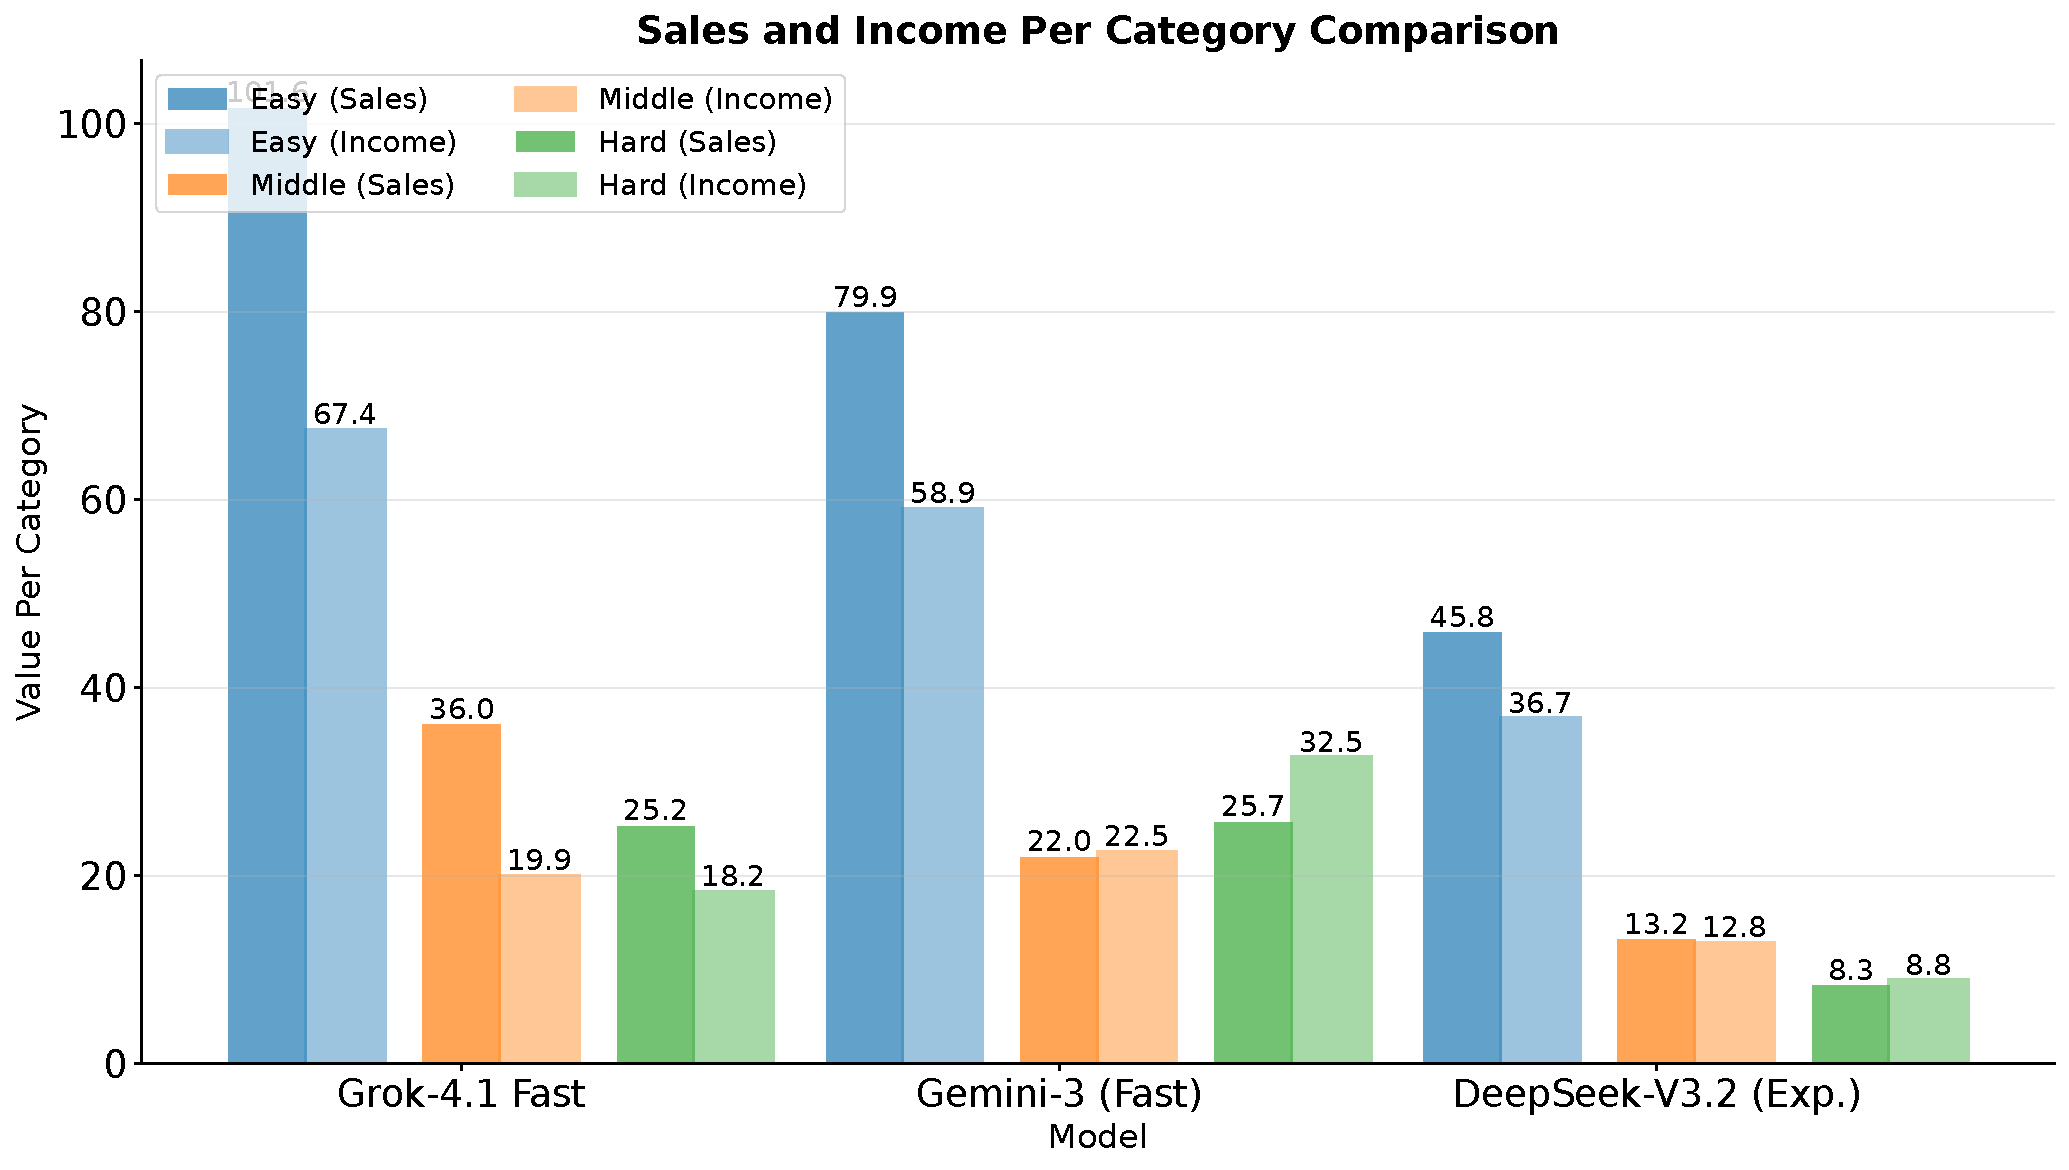
\includegraphics[width=1\linewidth]{figures/selected_models_metrics.pdf}
    \caption{Category-level sales and profit per category across Easy, Middle, and Hard environments. Results are shown for three representative models.}
    \label{fig:category_comparison}
\end{figure}

\subsection{Performance across Environments with Varying Difficulty}
As environment difficulty increases, all models exhibit consistent performance degradation in our experiments, including shorter operational durations, higher expiry and return ratios, and reduced long-horizon stability. Although the expansion of product categories in the Middle and Hard settings enables higher aggregate sales and profit for some models, \emph{Sales per Category} and \emph{Profit per Category} decline substantially (Figure~\ref{fig:category_comparison}). This pattern suggests challenges in resource allocation as decision spaces expand, though further investigation with additional seeds is needed to assess statistical significance.

The relatively small performance gap between the Middle and Hard environments can be partly attributed to the delayed impact of intensified news dynamics, whose effects typically unfold over longer time horizons. Appendix~\ref{appendix:total_results} reports the full results across all environments under the proposed framework. Overall, while models demonstrate limited adaptability as task complexity increases, their performance remains substantially below the heuristic upper bound, highlighting persistent limitations in robust long-horizon decision-making under complex and dynamic conditions.